
%%%%%%%%%%%%%%%%%%%%%%% file typeinst.tex %%%%%%%%%%%%%%%%%%%%%%%%%
%
% This is the LaTeX source for the instructions to authors using
% the LaTeX document class 'llncs.cls' for contributions to
% the Lecture Notes in Computer Sciences series.
% http://www.springer.com/lncs       Springer Heidelberg 2006/05/04
%
% It may be used as a template for your own input - copy it
% to a new file with a new name and use it as the basis
% for your article.
%
% NB: the document class 'llncs' has its own and detailed documentation, see
% ftp://ftp.springer.de/data/pubftp/pub/tex/latex/llncs/latex2e/llncsdoc.pdf
%
%%%%%%%%%%%%%%%%%%%%%%%%%%%%%%%%%%%%%%%%%%%%%%%%%%%%%%%%%%%%%%%%%%%



\documentclass[runningheads,a4paper]{llncs}

\usepackage{amssymb}
\setcounter{tocdepth}{3}
\usepackage{graphicx}

\usepackage{url}
\usepackage{listings}
\usepackage{amsmath}

\usepackage{array} % and/or
\usepackage{hyperref}

\urldef{\mailsa}\path|{alfred.hofmann, ursula.barth, ingrid.haas, frank.holzwarth,|
\urldef{\mailsb}\path|anna.kramer, leonie.kunz, christine.reiss, nicole.sator,|
\urldef{\mailsc}\path|erika.siebert-cole, peter.strasser, lncs}@springer.com|    
\newcommand{\keywords}[1]{\par\addvspace\baselineskip
\noindent\keywordname\enspace\ignorespaces#1}

\newcommand{\LJoin}{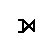
\includegraphics[scale=1.0]{img/ljoin}}

\newcommand{\superscript}[1]{\ensuremath{^{\textrm{#1}}}}
\newcommand{\subscript}[1]{\ensuremath{_{\textrm{#1}}}}

\newcommand{\rtwoo}{\textsf{R\subscript{2}O}}
\newcommand{\stwoo}{\textsf{S\subscript{2}O}}
\newcommand{\sparqlstr}{SPARQL\subscript{STR}}


\begin{document}

\mainmatter  % start of an individual contribution

% first the title is needed
\title{Ontology-based Access to Streaming Data}

% a short form should be given in case it is too long for the running head
\titlerunning{Ontology-based Access to Streaming Data}

% the name(s) of the author(s) follow(s) next
%
% NB: Chinese authors should write their first names(s) in front of
% their surnames. This ensures that the names appear correctly in
% the running heads and the author index.
%
\author{Jean-Paul Calbimonte$^1$, Oscar Corcho$^1$, and Alasdair J G Gray$^2$}
%
\authorrunning{Ontology-based Access to Streaming Data}
% (feature abused for this document to repeat the title also on left hand pages)

% the affiliations are given next; don't give your e-mail address
% unless you accept that it will be published
\institute{$^1$Ontology Engineering Group, Universidad Polit\'{e}cnica de Madrid, Spain\\ %Campus de Montegancedo s/n 28660, Boadilla del Monte, Spain\\
\email{jp.calbimonte@upm.es,ocorcho@fi.upm.es}\\
$^2$School of Computer Science, The University of Manchester, United Kingdom\\
%Oxford Road, Manchester M13 9PL, United Kingdom\\
\email{a.gray@cs.man.ac.uk}\\}
%
% NB: a more complex sample for affiliations and the mapping to the
% corresponding authors can be found in the file "llncs.dem"
% (search for the string "\mainmatter" where a contribution starts).
% "llncs.dem" accompanies the document class "llncs.cls".
%

\toctitle{Lecture Notes in Computer Science}
\tocauthor{Authors' Instructions}
\maketitle

\vspace{-10pt}
\begin{abstract}
The availability of streaming data sources is progressively increasing thanks to the development of ubiquitous data capturing technologies such as sensor networks. The heterogeneity of these sources introduces the requirement of providing data access in a unified and coherent manner. We present an ontology-based streaming data access service, based on extensions to the \rtwoo\ mapping language and its query processor ODEMapster, and to the C-SPARQL RDF stream query language. A preliminary implementation of the approach is also presented. With this proposal we expect to set the basis for future efforts in ontology-based streaming data integration.

%\keywords{Streaming data access, Ontology-based data access}
\end{abstract}

\lstdefinelanguage{SPARQLSTR}[]{SQL}{
morekeywords={STREAM,PREFIX, WINDOW, RANGE, SLIDE, AGGREGATE, AVG, STEP, REGISTER , QUERY},
sensitive=true,%
morecomment=[l]\#,%
morestring=[b]',%
}



\lstdefinestyle{SPARQLSTRStyle}{basicstyle=\sffamily\scriptsize,
                        %keywordstyle=\lstuppercase,
                        emphstyle=\itshape,
                        showstringspaces=false,
                        tabsize=2,
                        }

\lstdefinelanguage{R2O}{
morekeywords={streamschema,desc,name,has,stream,streamType,documentation,timestamp, keycol,nonkeycol,columnType,conceptmap,def,uri,as,virtualStream,described,by,
attributemap,has,column,applies,if,operation,dbrelationmap,toConcept,joins,via,condition},
sensitive=true,%
morecomment=[l]\#,%
morestring=[b]',%
}



\lstdefinestyle{HaskellSNEE}{basicstyle=\ttfamily\scriptsize,
                        %keywordstyle=\lstuppercase,
                        emphstyle=\itshape,
                        showstringspaces=false,
                        }

\lstdefinestyle{R2OStyle}{basicstyle=\sffamily\scriptsize,
                        %keywordstyle=\lstuppercase,
                        emphstyle=\itshape,
                        showstringspaces=false,
                        tabsize=2,
                        }

\section{Introduction}
\label{intro}

%Recent advances in wireless communications and sensor technologies have opened the way for deploying networks of interconnected sensing devices capable of ubiquitous data capture, processing and delivery. 
%Sensor network deployments are expected to increase significantly in the upcoming years because of their advantages and unique features. Tiny sensors can be installed virtually anywhere and still be reachable thanks to wireless communications. 
%Moreover, these devices are inexpensive and can be used for a wide range of applications such as security surveillance, traffic control, environmental monitoring, healthcare provision, industrial monitoring, etc.\
%One of the means to access streaming data sources coming from sensor networks is through query processors~\cite{Madden_05},\cite{Arasu_06a},\cite{Galpin_09} that handle streaming data %(which differs significantly from classical stored data, as it is potentially infinite and transient, with tuples being constantly added) 
%and support declarative continuous query languages. %(for which query results are updated regularly as time passes~\cite{Terry_92}).

In the context of the Semantic Web vision, several initiatives that aim at providing semantic access to traditional
(stored) data sources have been launched in the past years. Most of the existing approaches attempt to provide mappings
between the elements in the relational and ontological models \cite{Sahoo_09}.%, as we will describe in Section \ref{previousworks}. 
However, similar solutions for streaming data mapping and querying using ontology-based approaches have not been explored yet in depth. This has become especially relevant due to the emergence of sources such as sensor networks, capable of ubiquitous data capture, processing and delivery.

%In this paper we focus on providing ontology-based access to streaming data sources. Our apporach answers the requirements of i) establishing mappings between ontological models and streaming data source schemas, and ii) accessing streaming data sources through declarative continuous queries over ontology models. This constitutes a first step towards a framework for the integration of distributed heterogeneous streaming and stored data sources through ontological models. %and to the provision of Linked Data for streams~\cite{LePhuoc_09,Page_09,Sequeda_09}. 

%The paper is organised as follows: in Section \ref{previousworks} we introduce previous work. The foundations of our approach are explained in Section \ref{approach}. In Section \ref{syntax} we present the syntactic extensions for RDF stream SPARQL operators, and \rtwoo\ stream-to-ontology mappings. The semantics of these extensions are detailed in Section \ref{semanticsstreaming} and a first implementation of the execution of the streaming data access approach is explained in Section \ref{execution}. Finally we present the conclusions and future work.

\section{Ontology-based Streaming Data Access}
\label{approach}
% lightweight description, architecture
% include graphic
% contributions

%Querying streaming data and ontology-based access to stored data sources have already been studied by the research community and concrete proposals and software have been produced to deal with them. 

%\begin{itemize}
%\item establishing mappings between global ontological models and streaming data source schemas.
%\item accessing streaming data sources through queries over ontology global models.
%\item integrating streaming and stored data sources through an ontological unified view.
%\item combining data from event-based streams and/or sensor networks acquisitional streams considering time and tuple windows.
%\item considering quality-of-service requirements for query optimisation and source selection during the integration.
%\end{itemize}

Our approach consists in creating an Ontology-based Streaming Data Access service, depicted in Fig~\ref{fig:SemanticIntegrator}.\ %  that can receive requests over an ontological view and transforms them into queries for acquisitional or event-based stream sources or stored sources. The results of these queries can be integrated following a query plan and returned as RDF triples in terms of the global ontology. The approach is depicted in Fig ~\ref{fig:SemanticIntegrator}.
The service receives \sparqlstr queries specified in terms of 
%the classes and properties
%\footnote{We use the OWL nomenclature of classes and object and datatype properties for naming ontology elements.} 
of an ontology.
% using extensions of SPARQL that support operators over RDF streams and windows (\sparqlstr). 
Then the original query is transformed into queries in terms of the sources (\textit{query canonisation}), using 
%in order to transform the query in terms of the ontology into queries in terms of the sources, 
a set of \stwoo mappings. These are based on the \rtwoo\ mapping language, which has been extended to support  streaming queries and data, most notably window and stream operators. 
%This transformation process is called \textit{query canonisation}, and 
The transformed queires are written in a continuous query language (e.g. SNEEql), that is expressive enough to deal with both streaming and stored sources, and to apply window, aggregates and window-to-stream operations.

%After the continuous query has been generated, 
Afterwards, the query processing phase starts, and the processor will deploy distributed query processing techniques~\cite{Kossmann_00} to extract the relevant data from the sources and perform the required operations.
%creating a query plan that indicates how the sources will be accessed and how the data will be joined and combined using the available operators\cite{Kossmann_00}.
%
%Note that the execution in sources such as sensor networks may include in-network query processing, pull or push based data delivery and other data source specific settings. 
The result of the query processing will be a set of tuples that will be passed to a \textit{data decanonisation} process, which will transform these tuples to ontology instances.

%As it can be seen, this approach requires several contributions and extensions to the existing technologies for continuous data querying, ontology-based data access and SPARQL query processing. 
%This work focuses on a first stage that includes the process of transforming the SPARQL extended queries into queries over the streaming data sources using a language such as SNEEql as the target. 
%In the next sections a description of the query and mapping extensions syntax and semantics will be detailed, and afterwards we will provide results of an implementation of this approach.


\begin{figure}[here]
\vspace{-20pt} \hspace{20pt}
\begin{center}
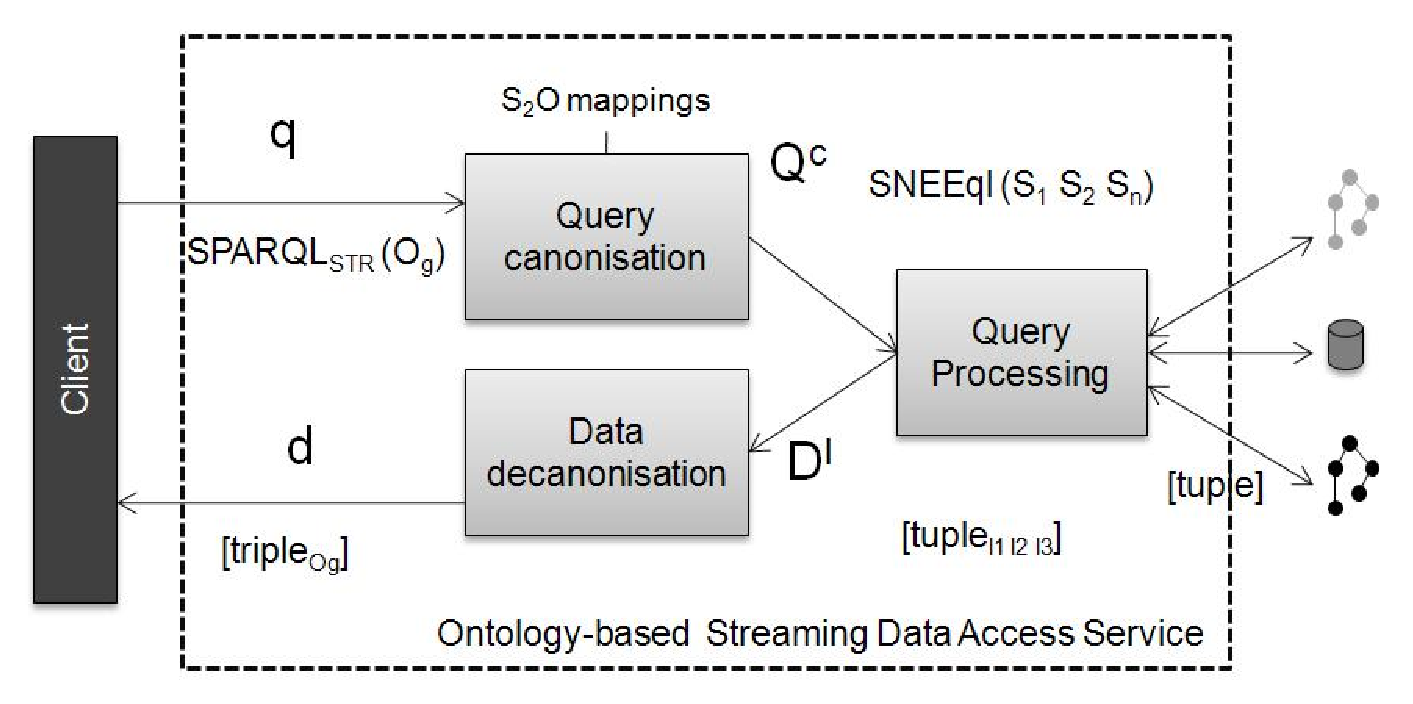
\includegraphics[width=8 cm]{img/approach}
\end{center}
\vspace{-10pt} \caption{Ontology-based Streaming Data Access service} \label{fig:SemanticIntegrator} \vspace{-20pt}
\end{figure}



\section{Implementation and Walkthrough}
\label{execution}

The presented approach of providing ontology-based access to streaming data has been implemented as an extension to the
ODEMapster processor \cite{Barrasa_04}. This implementation generates queries that can be executed by the SNEE streaming query processor using the SNEEql query language \cite{Brenninkmeijer_08}.

In the example, consider a stream \texttt{windsamples} and a table \texttt{sensors}, and the \stwoo mapping to a \textit{WindSpeedMeasurement} concept:
%Then we can define an \stwoo\ mapping that splits the \texttt{windsamples} stream tuples into instances of two different concepts $WindSpeedMeasurement$ and \textit{WindDirectionMeasurement}. Here is an extract of the \stwoo\ mapping concerning the $WindSpeedMeasurement$.

\begin{figure}[here]
\vspace{-20pt} \hspace{20pt}
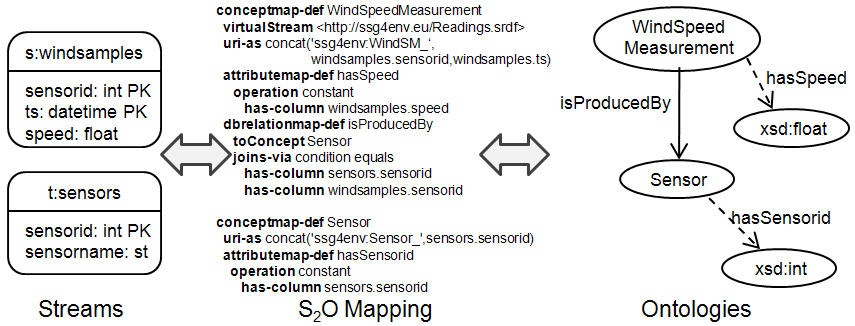
\includegraphics[width=10 cm]{img/mapping}
\vspace{-10pt} \caption{\stwoo\ mapping from stream to ontologies} \label{fig:Mappings} \vspace{-10pt}
\end{figure}

%The mapping extract here defines how to construct the $WindSpeedMeasurement$ ($WindSM$) and $Sensor$ class instances from the \texttt{windsamples} stream and the \texttt{sensors} table: $\Psi_{WindSM}\leadsto \Phi_{\mathtt{windsamples}}$ and $\Psi_{Sensor}\leadsto \Phi_{\mathtt{sensors}}$. In the case of the $WindSpeedMeasurement$ the function $f_{WindSM}^{Id}$ produces the URI's of the instances by concatenating the \texttt{sensorid} and \texttt{ts} attributes.
%explain the rest of the expression
Now we can pose a query over the ontology using \sparqlstr\, for example to obtain the wind speed measurements taken in the last 10 minutes:
%
\begin{lstlisting}[style=SPARQLSTRStyle,language=SPARQLSTR,frame=none]
PREFIX fire: <http://www.ssg4env.eu#>
PREFIX rdf: <http://www.w3.org/1999/02/22-rdf-syntax-ns#>
SELECT ?speed
FROM STREAM <www.ssg4env.eu/SensorReadings.srdf> [RANGE 10 MINUTE STEP 1 MINUTE]
WHERE { ?WindSpeed a fire:WindSpeedMeasurement; fire:hasSpeed ?speed;}
\end{lstlisting}
%
A class query atom $WindSpeedMeasurement(x)$ and a datatype property atom $hasSpeed(x,z)$ can be extracted from the \sparqlstr\ query. The window specification $[t_i=now-10,t_f=now,\delta=1,unit=minutes]$ is also obtained. As it is defined in the \stwoo\ mapping the $WindSpeedMeasurment$ instances are generated based on the \texttt{sensorid} and \texttt{ts} attributes of the \texttt{windsamples} stream.
%, using a concatenation function to generate each instance URI.
% Hence the processor will evaluate
%\begin{align*}
%\lambda(\Phi_{\mathtt{windsamples}}(x_{\mathtt{sensorid}},x_{\mathtt{ts}}))[now-10,now,1]) %= \\ \pi_{\mathtt{sensorid,ts}}(\omega_{now-10,now,1}\mathtt{windsamples})
%\end{align*}
Similarly the \stwoo\ mapping defines that $hasSpeed$ properties are generated from the values of the speed attribute of the \texttt{windsamples} stream. 
%The processor will evaluate this as:
%\begin{align*}
%\lambda(\Phi_{\mathtt{windsamples}}(x_{\mathtt{sensorid}},x_{\mathtt{ts}},z_{\mathtt{speed}})[now-10,now,1]) = \\ \pi_{\mathtt{sensorid,ts,speed}}(\omega_{now-10,now,1} \mathtt{windsamples})
%\end{align*}
%In this case no joins and other selection conditions are needed, and only one stream has to be queried to produce the results. 
The query generated in the SNEEql language is the following:
%\footnote {Although the current available implementation of the SNEE processor lacks the \texttt{concat} operator, we include the sample query in its complete form here.}:

\begin{lstlisting}[style=HaskellSNEE,language=SQL,frame=none]
SELECT RSTREAM concat('http://ssg4env.eu#WindSM',windsensor.id,windsensor.ts )
as  id ,( windsamples.speed ) as  speed
FROM windsamples[FROM NOW - 10 MINUTE]
\end{lstlisting}
%
The results will be transformed into tagged triples, instances of the class \\ $WindSpeedMeasurement$.


%\begin{lstlisting}[style=HaskellSNEE,language=Haskell,frame=none]
%windsamples: (sensorid INT PK,ts DATETIME PK,speed FLOAT,direction FLOAT)
%sensors: (sensorid INT PK,sensorname CHAR(45))
%\end{lstlisting}
%And consider the following ontological view:
%\begin{align*}%[style=HaskellSNEE,language=Haskell,frame=none]
%SpeedMeasurement \sqsubseteq\ & Measurement \\
%WindSpeedMeasurement \sqsubseteq\ & SpeedMeasurement \\
%WindDirectionMeasurement \sqsubseteq\ & Measurement \\
%SpeedMeasurement \sqsubseteq\ & \exists hasSpeed \\
%Measurement \sqsubseteq\ & \exists isProducedBy.Sensor \\
%Sensor \sqsubseteq\ & \exists hasName
%\end{align*}
%

%\lstdefinestyle{R2O}{basicstyle=\sffamily\scriptsize,
                        %keywordstyle=\lstuppercase,
%                        emphstyle=\itshape,
%                        showstringspaces=false,
%                        }
%\begin{lstlisting}[style=R2OStyle,language=R2O,frame=none]
%conceptmap-def WindSpeedMeasurement
% virtualStream <http://ssg4env.eu/SensorReadings.srdf>
% uri-as concat('ssg4env:WindSM_',windsamples.sensorid,windsamples.ts)
% described-by
%  attributemap-def hasSpeed
%   operation constant
%     has-column windsamples.speed
%  dbrelationmap-def isProducedBy toConcept Sensor
%   joins-via condition equals
%      has-column sensors.sensorid
%      has-column windsamples.sensorid
%
%conceptmap-def Sensor
% uri-as concat('ssg4env:Sensor_',sensors.sensorid)
% described-by
%  attributemap-def hasSensorid
%   operation constant
%     has-column sensors.sensorid
%\end{lstlisting}
%



%Show transformation example, mention implementation in infancy.
%We need to code at this point and show minimal results.


%\phantomsection
%\addcontentsline{toc}{section}{References}
\bibliographystyle{splncs}
\bibliography{re}



\end{document}
